\documentclass{article}
\usepackage{neurips_2026}
\usepackage[utf8]{inputenc}
\usepackage[T1]{fontenc}
\usepackage{hyperref}
\usepackage{url}
\usepackage{booktabs}
\usepackage{amsfonts,amsmath,amssymb,amsthm}
\usepackage{nicefrac}
\usepackage{microtype}
\usepackage{xcolor}
\usepackage{graphicx}

\newtheorem{proposition}{Proposition}
\newcommand{\nloc}{n_{\rm loc}}
\newcommand{\thh}{\hat\theta}

\title{How Many Comparisons Does It Take to Flip a Leaderboard? Scale-Free Sensitivity of Bradley--Terry Rankings Across Evaluation Designs}

\author{Anonymous Authors}

\begin{document}
\maketitle

\begin{abstract}
Leaderboards built from pairwise comparisons (crowd votes, expert or model judges, sports results) are fitted with Bradley--Terry (BT) models and read as rankings. We ask how many comparisons must be \emph{changed}---by noise or by an adversary---to flip the BT order of two contestants, and whether the answer depends on the evaluation design. We define the budget of a pair as the number of comparisons that a greedy adversary with exact refitting must remove, relabel or insert, and normalise it by the number of comparisons involving the two contestants. On four designs (Chatbot Arena crowd votes, MT-Bench human experts, MT-Bench GPT-4 judge, 16 NBA seasons) we find: (i) in dense leaderboards most adjacent orders are not statistically resolved and flip with at most 5 edits (62\% of adjacent Arena pairs, 98\% of NBA pairs), whereas the well-separated MT-Bench pairs need 2--6\% of their local comparisons; (ii) the \emph{fraction} of local comparisons needed is proportional to the BT score gap, $f\approx\kappa\,\Delta\theta$ with $\kappa\approx0.06$ for relabelling (0.08 for NBA) and $\approx0.12$ for removal, nearly constant across designs and across a 32-fold change of the Arena sample size; equivalently, the edit \emph{count} is about $0.2\,z\sqrt{\nloc}$ for $z$-score $z$; (iii) a crowd-vs-expert control on six matched models at matched size shows no detectable design effect beyond gap and size; (iv) random removals of the same size never flipped a pair that needs $\geq5$ targeted edits. Designs thus differ mainly in how densely contestants are packed relative to noise, not in intrinsic fragility per unit of score. We state the conditions and limits of these conclusions.
\end{abstract}

\section{Introduction}
Model leaderboards that aggregate many ``A versus B, which is better?'' judgments are used for model selection, release announcements and research comparisons. Their rankings come from a Bradley--Terry (BT) fit \citep{bradley1952} to the comparison data, often with bootstrap confidence intervals, as on Chatbot Arena \citep{chiang2024}. What is much less clear is how strongly a published rank depends on the underlying comparisons, whether the change comes from honest noise, from a few corrupted records, or from deliberate manipulation \citep{min2025,singh2025}, and whether this dependence differs between evaluation designs: anonymous crowd voting, expert annotation, an LLM judge \citep{zheng2023}, or sports results.

This paper makes the question operational and answers it empirically.
\begin{itemize}
\item \textbf{Definition.} The \emph{edit budget} $k(i,j)$ of an adjacent pair is the smallest number of unit edits (remove, relabel, or insert a comparison) found by a greedy adversary, with exact BT refitting, that reverses the estimated order of $i$ and $j$. To compare boards of different size we normalise by $\nloc$, the number of comparisons involving $i$ or $j$ (Sec.~\ref{sec:method}).
\item \textbf{Evidence.} Four designs from public data: Chatbot Arena crowd votes (64 models, 57{,}477 votes), MT-Bench human-expert and GPT-4-judge pairs (6 models), and 16 NBA regular seasons (about 30 teams, 1{,}230 games each). We also run a matched control (Arena votes restricted to the six MT-Bench models), subsampling, random-edit, and robustness experiments.
\item \textbf{Findings.} (a) Sensitivity is not one number per leaderboard: most adjacent pairs in dense boards are statistical ties and need $\leq5$ edits, while resolved pairs need a few percent of their local data. (b) The fraction of local comparisons needed is proportional to the BT gap with a design-independent constant to within a factor of about 1.4, and is independent of the amount of data. (c) Hence statistical resolution (a $z$-score) and robustness to a fractional adversary are different things: more data resolves more pairs but does not make a given gap harder to overturn in relative terms.
\end{itemize}
Our conclusions are conditional: they concern first-order-adjacent ranks in BT models fitted to the specific snapshots listed in Sec.~\ref{sec:data}; the adversary is a heuristic upper bound on the true minimum; and we do not model how a real attacker could realise the edits.

\section{Related work}
\textbf{Paired-comparison leaderboards.} The BT model \citep{bradley1952} underlies Chatbot Arena \citep{chiang2024}, which collects pairwise human votes and reports ranks with bootstrap intervals. MT-Bench \citep{zheng2023} provides expert human and GPT-4 pairwise judgments on 80 questions for six public models; we use both. \textbf{Manipulation and distortion.} \citet{min2025} study how voting strategies can raise or lower a model's Arena rank, and \citet{singh2025} document evaluation practices (private testing, unequal sampling) that distort the leaderboard. Our analysis is complementary: instead of a particular attack or practice we ask, for a fixed snapshot, how large \emph{any} edit set must be, and compare designs. \textbf{Data-removal robustness.} Influence functions \citep{koh2017} approximate how a model changes when training points are removed, and \citet{broderick2020} use such approximations to find the small data subset whose removal changes an applied conclusion (``Approximate Maximum Influence Perturbation''). We use the same linearisation to propose edits but refit exactly after each chunk, extend the edit set to relabelling and insertion, and apply it across evaluation designs. We did not consult every listed paper in full (App.~\ref{app:repro}); in particular we did not read the leaderboard-specific work on dropping preferences that appears in the task's reading list, so we make no priority claim relative to it.

\section{Method}\label{sec:method}
\textbf{Model.} A comparison $s$ between $a_s$ and $b_s$ has outcome $y_s\in\{1,\tfrac12,0\}$ (win for $a_s$, tie, win for $b_s$). Ties are counted as half a win each, as in Elo/BT leaderboards. We fit
$\thh=\arg\min_\theta -\sum_s [y_s\log\sigma(\theta_{a_s}-\theta_{b_s})+(1-y_s)\log\sigma(\theta_{b_s}-\theta_{a_s})]+\tfrac{\lambda}{2}\|\theta\|^2$ with $\lambda=10^{-3}$ (fixing the additive gauge; results are unchanged for $\lambda\in[10^{-5},1]$, App.~\ref{app:robust}) by Newton's method on pair-aggregated counts. Contestants are ranked by $\thh$; the Hessian is $H$.

\textbf{Pair sensitivity.} For ranks $r$ and $r{+}d$ ($d=1$ unless stated) with contestants $i,j$, gap $\Delta\thh=\th_i-\th_j>0$. A \emph{unit edit} is: \emph{remove} one comparison; \emph{relabel} one comparison to another outcome; or \emph{insert} one new comparison of any pair and outcome (rigging-style; not meaningful for fixed schedules such as the NBA, where we report it only for completeness). The budget $k_{\rm mode}(i,j)$ is the smallest number of edits found that makes $\th_i<\th_j$ after refitting.

\textbf{Greedy adversary.} Let $c=e_i-e_j$ and $v=H^{-1}c$. To first order, an edit of a comparison with design vector $x=e_a-e_b$ and fitted win probability $p$ changes the contrast $c^\top\theta$ by $v^\top x\,(p-y)$ (removal), $v^\top x\,(y'-y)$ (relabel $y\to y'$) or $v^\top x\,(y'-p)$ (insertion). Each round ranks all (pair, outcome) cells by predicted decrease, applies a chunk of $\max(1,\lfloor\tfrac12\,\text{margin}/\text{best gain}\rfloor)$ edits subject to cell counts, refits exactly, and stops when the order is reversed; chunks shrink to one edit near the end. Edits may touch any comparison, not only those of $i$ and $j$; $\nloc$ is just a normaliser (for insertions it is the original count). The returned $k$ is therefore an \emph{upper bound} on the true minimum. On 150 (removal) and 152 (relabel) random tiny instances (3 contestants, 20--39 votes) where exhaustive search was feasible, greedy matched the exact minimum in 96.7\% and 99.3\% of cases and never beat it; its worst ratio was 2.0 (App.~\ref{app:robust}).

\textbf{Normalisation across designs.} Raw counts depend on board size. We report (i) $f=k/\nloc$, where $\nloc=n_i+n_j-n_{ij}$ is the number of comparisons involving $i$ or $j$; (ii) the BT gap $\Delta\thh$ in logits; and (iii) the $z$-score $z=\Delta\thh/\hat\sigma_{ij}$, with $\hat\sigma_{ij}$ the standard deviation of $\th_i-\th_j$ over $B{=}200$ nonparametric bootstrap resamples of the votes. Two empirical constants summarise a design: $\kappa=f/\Delta\thh$ and $c=k/(z\sqrt{\nloc})$.

\begin{proposition}[First-order scale of the budget]\label{prop:scale}
Let $\sigma_c^2=c^\top H^{-1}c$ and $s_x^2=x^\top H^{-1}x$. If a set of edits $\{(x_s,\delta_s)\}$ reverses the pair in the linearisation, then $\sum_s|\delta_s|\,s_{x_s}\geq\Delta\thh/\sigma_c$.
\end{proposition}
\emph{Proof sketch.} The linearised change of $c^\top\theta$ is $\sum_s\delta_s\,c^\top H^{-1}x_s$; it must be at most $-\Delta\thh$. Since $H^{-1}\succeq0$, Cauchy--Schwarz gives $|c^\top H^{-1}x_s|\leq\sigma_c s_{x_s}$. \hfill$\square$

\noindent The proposition is only heuristic (the true map is nonlinear and $H^{-1}$ changes as edits are made) but explains the form of our empirical findings: a contrast with standard error $\sigma_c\propto1/\sqrt{\nloc}$ separated by $z$ standard errors needs an ``edit mass'' of at least $z$ in units of per-comparison standard errors, i.e.\ a count that grows like $z\sqrt{\nloc}$, and a \emph{fraction} $k/\nloc$ that grows like $\Delta\thh$ once $\sigma_c\sqrt{\nloc}$ is roughly constant.

\section{Data and protocol}\label{sec:data}
Table~\ref{tab:overview} lists the boards (sources, versions and checksums in App.~\ref{app:repro}). \textbf{Arena (crowd):} the 55k human-preference snapshot of Chatbot Arena, 64 models, 31\% ties (including ``both bad''). \textbf{MT-Bench (human):} 3{,}355 judgments by experts and authors on 80 two-turn questions; \textbf{MT-Bench (GPT-4 judge):} 2{,}400 GPT-4 pairwise verdicts on the same questions (``inconsistent'' verdicts counted as ties). \textbf{NBA (sports):} one board per regular season 2000--2015 (franchise level, no home-court term), chosen before looking at results as the 29--30-team era. The four designs differ in who judges, number of contestants (6 to 64), votes per contestant, tie rates, and how dense the ability scale is. Throughout, the MT-Bench boards have 6 contestants, so ``adjacent pairs'' there number only 5 each; their statistics are correspondingly coarse.

\textbf{Uncertainty.} Intervals for fractions and medians are percentile bootstrap intervals over pairs (over seasons' pairs for NBA, resampled by season). Bootstrap standard deviations $\hat\sigma_{ij}$ use $B=200$ vote-level resamples (question-clustered resampling is reported in App.~\ref{app:robust}). All randomness is seeded; the whole pipeline runs in a few minutes on CPU. \textbf{Exploratory vs.\ confirmatory.} The study design (boards, adversaries, normalisation by $\nloc$, $z$) was fixed before running. The proportionality $f\propto\Delta\thh$ and the constants $\kappa$ were identified post hoc from the main pair table; later subsampling and matched-control runs were analysed for $\kappa$ afterwards, so only the agreement across designs (not the subsample series, which reuses the same Arena votes) counts as a consistency check. Thresholds ($z\geq2$, $k\geq5$, $\Delta\thh>0.05$, $\epsilon\in\{0.5,1,2,5\}\%$) were set by us without pre-registration; $k\geq5$ and $\Delta\thh>0.05$ merely exclude pairs where integer rounding or near-zero gaps dominate. We report descriptive intervals, not hypothesis tests, so no multiple-testing correction is applied.

\begin{table}[t]
\caption{Boards studied. ``bootstrap $\tau$'': mean Kendall $\tau$ between the full-data ranking and bootstrap rankings; ``top-1 kept'': fraction of bootstrap fits with the same top contestant; last column: share of adjacent pairs with $z\geq2$ (bootstrap 95\% interval). NBA entries: median over 16 seasons (range).}\label{tab:overview}
\centering\scriptsize
\resizebox{\textwidth}{!}{\begin{tabular}{lrrrrlll}\toprule
 Design & \#boards & players & votes $N$ & ties & bootstrap $\tau$ & top-1 kept & adjacent pairs $z\geq2$ \\\midrule
Arena (crowd votes) & 1 & 64 & 57477 & 31\% & 0.92 & 0.47 & 6\% [2, 13] \\
MT-Bench (human) & 1 & 6 & 3355 & 23\% & 0.96 & 1.00 & 80\% [40, 100] \\
MT-Bench (GPT-4 judge) & 1 & 6 & 2400 & 25\% & 1.00 & 1.00 & 100\% [100, 100] \\
NBA (games) & 16 & 30 & 1230 & 0\% & 0.81 (0.76--0.83) & 0.50 (0.28--0.89) & 0\% [0, 1] \\
\bottomrule\end{tabular}
}
\end{table}

\section{Results}
\subsection{Most adjacent orders in dense boards are inside the noise---and cost a handful of edits}
Table~\ref{tab:overview} shows how different the boards are statistically: 80--100\% of the adjacent MT-Bench pairs are resolved ($z\geq2$), but only 6\% (4 of 63) in Arena and 0.2\% (1 of 459) in NBA. The Arena leader is not resolved either: \texttt{gpt-4-1106-preview} and \texttt{gpt-4-0125-preview} differ by $0.004$ logits, and the top-1 identity survives only 47\% of bootstrap fits (NBA: 50\%, range 28--89\%).

Table~\ref{tab:fragility} reports the share of adjacent pairs flippable by relabelling at most a fraction $\epsilon$ of their local votes. At $\epsilon=1\%$ this is 97\% of Arena pairs and 68\% of NBA pairs, but 20\% and 0\% for the two MT-Bench boards; by $\epsilon=5\%$ nearly everything flips (MT-Bench: 4 of 5 pairs). In absolute terms $k_{\rm relabel}\leq5$ for 62\% of Arena and 98\% of NBA adjacent pairs and for none of the MT-Bench pairs. Restricting to resolved pairs ($z\geq2$, lower half of Table~\ref{tab:fragility}) changes the picture: the 4 resolved Arena pairs need 0.5--2\% of local votes (e.g.\ \texttt{gpt-4-0125-preview} vs \texttt{gpt-4-0314}: 105 relabels among 5{,}265 local votes, $z=7.7$) and resolved MT-Bench pairs need 2.5--6\%. The single resolved NBA pair (Wizards, 2012) needs about 8\%. Table~\ref{tab:leader} gives the leader: in MT-Bench, dethroning GPT-4 needs 46 (human) or 61 (GPT-4 judge) relabels, 2.5\% and 4.2\% of its local comparisons; the BT-top team of the median NBA season is overtaken by 2 relabels (range 0--8), and in 12 of 16 seasons has $z<1$ over the runner-up.

\begin{table}[t]
\caption{Share (\%) of adjacent pairs that a relabelling adversary can flip using at most a fraction $\epsilon$ of the votes involving the two contestants. 95\% bootstrap intervals; tiny $n$ (MT-Bench: 5 pairs) makes the intervals wide.}\label{tab:fragility}
\centering\scriptsize
\resizebox{\textwidth}{!}{\begin{tabular}{llcccc}\toprule
 Design & pairs & $\epsilon$=0.5\% & $\epsilon$=1\% & $\epsilon$=2\% & $\epsilon$=5\% \\\midrule
Arena (crowd votes) & all adjacent ($n$=63) & 84 [75,92] & 97 [92,100] & 100 [100,100] & 100 [100,100] \\
MT-Bench (human) & all adjacent ($n$=5) & 20 [0,60] & 20 [0,60] & 20 [0,60] & 80 [40,100] \\
MT-Bench (GPT-4 judge) & all adjacent ($n$=5) & 0 [0,0] & 0 [0,0] & 0 [0,0] & 80 [40,100] \\
NBA (games) & all adjacent ($n$=453) & 0 [0,0] & 68 [65,71] & 94 [92,96] & 100 [99,100] \\
\midrule
Arena (crowd votes) & $z\geq2$ ($n$=4) & 0 [0,0] & 50 [0,100] & 100 [100,100] & 100 [100,100] \\
MT-Bench (human) & $z\geq2$ ($n$=4) & 0 [0,0] & 0 [0,0] & 0 [0,0] & 75 [25,100] \\
MT-Bench (GPT-4 judge) & $z\geq2$ ($n$=5) & 0 [0,0] & 0 [0,0] & 0 [0,0] & 80 [40,100] \\
NBA (games) & $z\geq2$ ($n$=1) & 0 [0,0] & 0 [0,0] & 0 [0,0] & 0 [0,0] \\
\bottomrule\end{tabular}
}
\end{table}
\begin{table}[t]
\caption{The top-ranked contestant vs.\ rank 2: gap, bootstrap $z$, local votes, and edits needed to reverse (relabel / remove). NBA: median over seasons (range).}\label{tab:leader}
\centering\scriptsize
\resizebox{\textwidth}{!}{\begin{tabular}{lrrrrrr}\toprule
 Board & gap $\hat\theta_1-\hat\theta_2$ & $z$ & $n_{\rm loc}$ & $k_{\rm relabel}$ & $k_{\rm remove}$ & $k_{\rm relabel}/n_{\rm loc}$ \\\midrule
Arena (crowd votes) & 0.00 & 0.1 & 8413 & 1 & 2 & 0.01\% \\
MT-Bench (human) & 0.38 & 4.8 & 1825 & 46 & 92 & 2.52\% \\
MT-Bench (GPT-4 judge) & 0.82 & 8.7 & 1440 & 61 & 143 & 4.24\% \\
NBA (games) & 0.15 (0.00--0.62) & 0.4 (0.0--1.5) & 160 (131--162) & 2 (0--8) & 3 (0--9) & 1.39 (0.00--4.94)\% \\
\bottomrule\end{tabular}
}
\end{table}

\subsection{A scale-free regularity: the fraction of votes to edit is proportional to the gap}
Figure~\ref{fig:law}(a) plots $f=k_{\rm relabel}/\nloc$ against the gap for every adjacent pair of every board. Above the integer floor $f\geq1/\nloc$ (visible for NBA and near-ties), the points follow a line through the origin in log--log coordinates: for pairs with $\Delta\thh>0.05$ and $k\geq5$ (42 pairs), a log--log regression has slope $1.06$ (95\% cluster-bootstrap interval $[0.43,1.15]$) for relabelling, $1.01$ $[0.68,1.05]$ for removal and $1.03$ $[0.73,1.07]$ for insertion, with residual sd 0.29 in $\log f$. The proportionality constants, Table~\ref{tab:kappa}, are $\kappa_{\rm relabel}\approx0.06$ (Arena 0.059, MT-Bench human 0.067, GPT-4 judge 0.056, NBA 0.082), $\kappa_{\rm remove}\approx0.11$--$0.14$ and $\kappa_{\rm insert}\approx0.10$--$0.13$. Interpreted: to reverse a gap of $0.3$ logits (about a 7-point win-probability difference near $\tfrac12$), an adversary must relabel about 1.8\% of the votes involving the two contestants, removal needs about twice as many edits (median ratio relabel/remove $0.60$, 10--90\% range $0.46$--$0.71$) and insertion about 0.9 of the removal cost. Design differences in $\kappa$ are at most a factor of 1.5 (NBA vs.\ MT-Bench GPT-4), and the NBA value is the only one clearly outside the others' intervals; we do not have a tested explanation for it (a test of the hypothesis that ties explain the difference, by dropping ties, did not support it, App.~\ref{app:robust}).

\begin{figure}[t]
\centering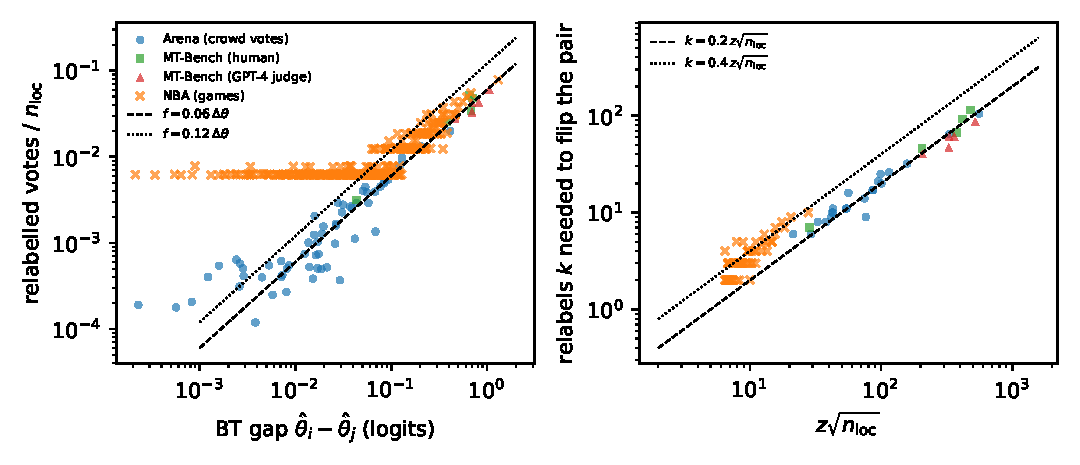
\includegraphics[width=\textwidth]{figures/fig_law.pdf}
\caption{(a) Fraction of local votes relabelled to flip an adjacent pair vs.\ BT gap, all pairs of all boards (453 NBA, 63 Arena and 5+5 MT-Bench pairs; 6 NBA pairs with identical fitted scores are omitted). The horizontal run at $f\approx6\times10^{-3}$ is the one-edit floor for NBA. (b) Number of relabels vs.\ $z\sqrt{\nloc}$ for pairs with $z\geq0.5$.}\label{fig:law}
\end{figure}
\begin{table}[t]
\caption{$\kappa=f/\Delta\thh$, the fraction of the contestants' votes to edit per logit of gap, median over pairs with $\Delta\thh>0.05$ and $k_{\rm relabel}\geq5$ (95\% bootstrap interval).}\label{tab:kappa}
\centering\scriptsize
\resizebox{0.8\textwidth}{!}{\begin{tabular}{lrccc}\toprule
Design & pairs & $\kappa_{\rm relabel}$ & $\kappa_{\rm remove}$ & $\kappa_{\rm insert}$ \\\midrule
Arena (crowd votes) & 18 & 0.059 [0.058, 0.064] & 0.116 [0.111, 0.134] & 0.105 [0.093, 0.116] \\
MT-Bench (human) & 4 & 0.067 [0.050, 0.078] & 0.142 [0.106, 0.157] & 0.134 [0.100, 0.156] \\
MT-Bench (GPT-4 judge) & 5 & 0.056 [0.047, 0.061] & 0.123 [0.095, 0.150] & 0.113 [0.094, 0.122] \\
NBA (games) & 15 & 0.082 [0.074, 0.096] & 0.112 [0.101, 0.124] & 0.101 [0.097, 0.117] \\
\bottomrule\end{tabular}
}
\end{table}

\textbf{Link to statistical resolution.} Combining $f=\kappa\Delta\thh$ with $\Delta\thh=z\hat\sigma_{ij}$ predicts $k=c\,z\sqrt{\nloc}$ if $\hat\sigma_{ij}\sqrt{\nloc}$ is roughly constant. It is: its median is 3.7 (Arena), 3.4 (MT-Bench human), 3.1 (GPT-4 judge), 4.5 (NBA). Figure~\ref{fig:law}(b) confirms $k\approx c\,z\sqrt{\nloc}$ over almost three decades with $c_{\rm relabel}$ (median, $z\geq1$) equal to 0.20, 0.22, 0.17 and 0.38 for the four designs and $c_{\rm remove}$ of 0.40, 0.46, 0.42 and 0.54 (intervals in App.~\ref{app:robust}). A pooled regression of $\log k_{\rm relabel}$ on $\log z$ and $\log\nloc$ (36 pairs with $z\geq1$) gives exponents $0.89$ on $z$ ($[0.75,1.29]$) and $0.32$ on $\nloc$ ($[0.15,1.80]$); for removal $0.97$ ($[0.78,1.05]$) and $0.42$ ($[-0.04,0.49]$). The $\sqrt{\nloc}$ exponent is thus imprecisely determined (the 36 pairs vary mostly in $z$), and the exponent 0.5 is consistent with removal but at the edge for relabelling.

\subsection{Rank displacement and random versus targeted edits}
Moving a contestant $d$ places down costs more roughly linearly in $d$ (Figure~\ref{fig:shift}, left): the median relabel fraction for $d=1$ vs.\ $d=5$ is 0.10\% vs.\ 0.75\% (Arena), 3.4\% vs.\ 22\% (MT-Bench human), 4.2\% vs.\ 30\% (GPT-4 judge) and 0.63\% vs.\ 3.7\% (NBA). Pushing GPT-4 from first to last place in MT-Bench takes 423 (human) and 430 (GPT-4 judge) relabels, i.e.\ 22\% and 30\% of its local votes against the last-ranked model.

\begin{figure}[t]
\centering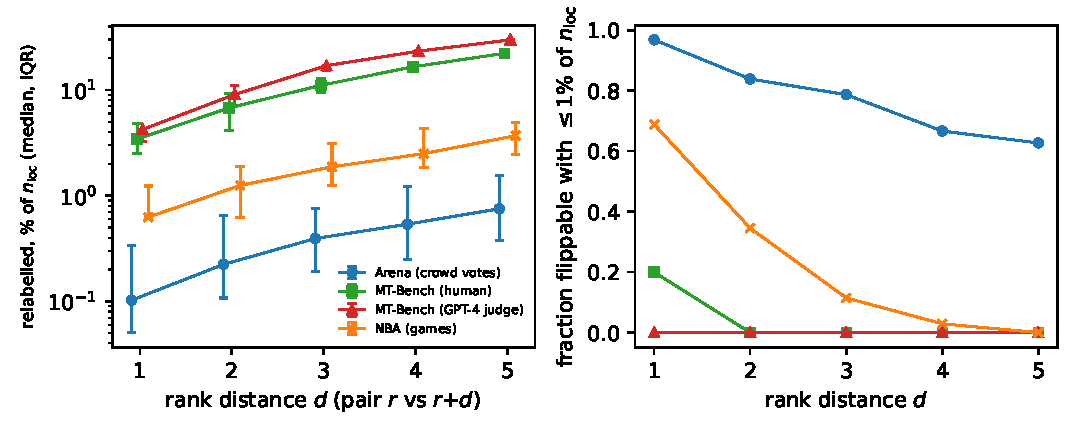
\includegraphics[width=0.49\textwidth]{figures/fig_rankshift.pdf}\hfill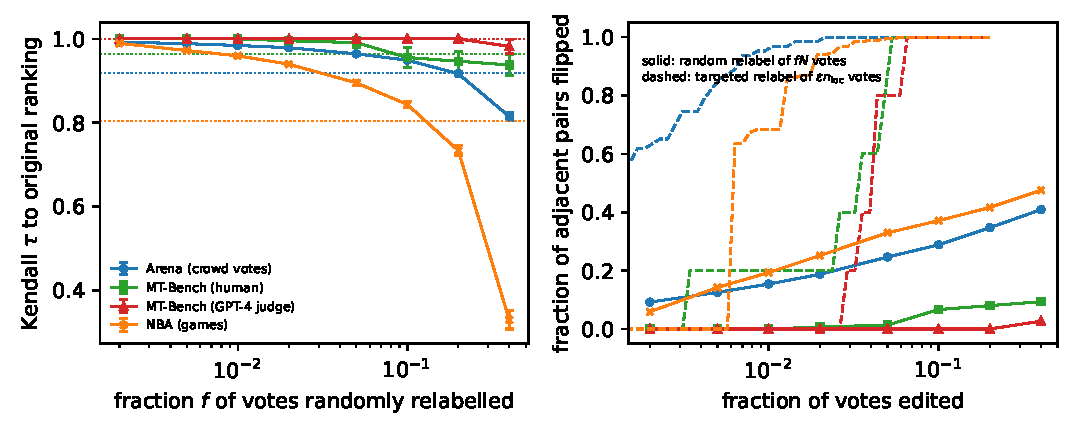
\includegraphics[width=0.49\textwidth]{figures/fig_noise.pdf}
\caption{Left: cost of displacing a contestant by $d$ ranks (median and interquartile range over pairs; right sub-panel: share flippable with $\leq1\%$ of local votes). Right: random relabelling of a fraction $f$ of all votes (mean Kendall $\tau$ to the original ranking, 95\% intervals over 30 repetitions, 5 per NBA season; dotted: bootstrap $\tau$) and fraction of adjacent pairs flipped, random (solid) vs.\ targeted (dashed, per-pair adversary).}\label{fig:shift}
\end{figure}
Random edits are far less damaging (Fig.~\ref{fig:shift}, right). Relabelling 1\% of all votes at random leaves Kendall $\tau$ at 0.984 (Arena), 1.00 (MT-Bench human/GPT-4) and 0.96 (NBA), while the sampling noise of the boards, as measured by bootstrap $\tau$, equals what random relabelling of roughly 8--20\% of the votes would produce (bootstrap $\tau$ Arena 0.92, NBA 0.80, MT-Bench human 0.96; the GPT-4-judge board has bootstrap $\tau=1.00$). Random removal of exactly the adversary's budget $k_{\rm remove}$ votes (50 repetitions per pair) flipped none of the 92 pairs with $k_{\rm remove}\geq5$ in any repetition; it flips only some of the pairs with near-zero gaps that need 1--4 edits. The share of adjacent pairs flipped by random 1\% relabelling is 15\% (Arena) and 19\% (NBA), i.e.\ these flips are essentially the pairs that are already coin flips under resampling (mean bootstrap flip probability 0.41 for $z<1$, 0.11 for $1\leq z<2$, 0.003 for $z\geq2$). Targeted edits thus do not create instability in dense boards; they exploit what resampling already leaves undecided and then, for resolved pairs, a few percent of local votes.

\subsection{Does more data help? Subsampling and a matched crowd-vs-expert control}
\textbf{Subsampling.} We keep a random $1/32,\dots,1/2$ of the Arena votes (10 repetitions each) and recompute everything. $\kappa_{\rm relabel}$ stays at 0.061--0.064 for kept fractions $1/32$ to $1/2$ (3 to 115 qualifying pairs per setting) and is 0.059 at full size, a 32-fold range (Figure~\ref{fig:sub}, left; the subsamples reuse the same votes, so this tests dependence on size, not independent replication), and $c_{\rm relabel}$ at 0.20--0.23, while the share of resolved adjacent pairs rises from 0.2\% to 6.3\%. More data therefore resolves more pairs but does not change the \emph{fraction} of votes needed per logit of gap; the absolute count grows in proportion to $\nloc$.

\begin{figure}[t]
\centering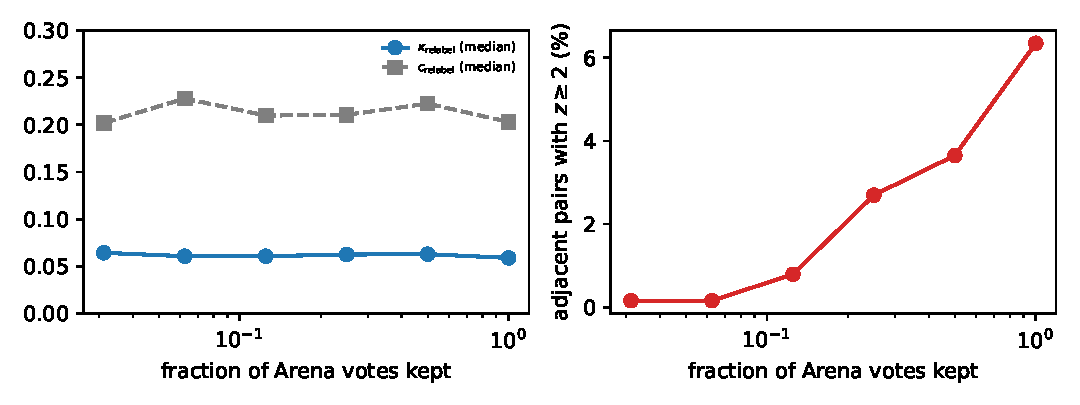
\includegraphics[width=0.7\textwidth]{figures/fig_subsample.pdf}
\caption{Arena votes subsampled. Left: median $\kappa_{\rm relabel}$ and $c_{\rm relabel}$. Right: share of adjacent pairs with $z\geq2$.}\label{fig:sub}
\end{figure}

\textbf{Matched control.} To separate evaluation design from board size and contestant set, we restrict Arena votes to six models that match the MT-Bench set (\texttt{gpt-4-0314}, \texttt{claude-1}, \texttt{gpt-3.5-turbo-0314}, \texttt{vicuna-13b}, \texttt{alpaca-13b}, \texttt{llama-13b}; versions are the nearest available, not identical), leaving 1{,}367 votes with 27\% ties, and subsample MT-Bench to the same size (30 repetitions). The BT scores of the two boards agree closely (e.g.\ gpt-4 1.09 vs.\ 1.02, llama-13b $-1.53$ vs.\ $-1.45$ for Arena-6 vs.\ MT-Bench human), though the crowd board separates claude-v1 from gpt-3.5-turbo more (0.34 vs.\ 0.04 logits). Table~\ref{tab:matched} shows the five adjacent pairs: the relabel fraction is 2.4--5.7\% (Arena-6, median $\kappa=0.071$), 2.5--4.9\% for MT-Bench human apart from a near-tied pair (median $\kappa=0.068$) and 2.8--6.0\% for the GPT-4 judge ($\kappa=0.057$). The three median $\kappa$ values lie within a factor of 1.25 of each other, smaller than the pair-to-pair spread inside the Arena-6 board (0.050--0.101). We conclude that, for these six models, crowd, expert and model-judge designs show no detectable difference in $\kappa$ or $c$ once gap and size are accounted for; this is one contestant set and one snapshot per design, with 5 pairs per board.

\begin{table}[t]
\caption{Matched control: Arena votes restricted to six models (1{,}367 votes) versus MT-Bench subsampled to 1{,}367 votes (mean over 30 subsamples; pair identity by rank).}\label{tab:matched}
\centering\scriptsize
\resizebox{\textwidth}{!}{\begin{tabular}{llrrrrr}\toprule
 Board & adjacent pair & gap & $z$ & $n_{\rm loc}$ & $k_{\rm relabel}$ & $k/n_{\rm loc}$ (\%) \\\midrule
Arena-6 (crowd, $N$=1367) & gpt-4 / claude-v1 & 0.30 & 3.5 & 882 & 27 & 3.1 \\
Arena-6 (crowd, $N$=1367) & claude-v1 / gpt-3.5-turbo & 0.34 & 3.3 & 872 & 21 & 2.4 \\
Arena-6 (crowd, $N$=1367) & gpt-3.5-turbo / vicuna-13b-v1.2 & 0.46 & 4.8 & 858 & 28 & 3.3 \\
Arena-6 (crowd, $N$=1367) & vicuna-13b-v1.2 / alpaca-13b & 0.76 & 7.5 & 865 & 49 & 5.7 \\
Arena-6 (crowd, $N$=1367) & alpaca-13b / llama-13b & 0.75 & 4.8 & 607 & 23 & 3.8 \\
\midrule
MT-Bench human, subsampled to 1367 & rank 1--2 & 0.37 & 3.2 & 800 & 20 & 2.5 \\
MT-Bench human, subsampled to 1367 & rank 2--3 & 0.07 & 0.6 & 908 & 4 & 0.5 \\
MT-Bench human, subsampled to 1367 & rank 3--4 & 0.64 & 6.2 & 872 & 42 & 4.8 \\
MT-Bench human, subsampled to 1367 & rank 4--5 & 0.71 & 6.5 & 776 & 38 & 4.9 \\
MT-Bench human, subsampled to 1367 & rank 5--6 & 0.69 & 5.4 & 793 & 28 & 3.6 \\
\midrule
MT-Bench GPT-4, subsampled to 1367 & rank 1--2 & 0.79 & 6.4 & 817 & 34 & 4.1 \\
MT-Bench GPT-4, subsampled to 1367 & rank 2--3 & 0.46 & 4.4 & 818 & 23 & 2.8 \\
MT-Bench GPT-4, subsampled to 1367 & rank 3--4 & 0.70 & 6.6 & 823 & 35 & 4.3 \\
MT-Bench GPT-4, subsampled to 1367 & rank 4--5 & 1.05 & 9.3 & 823 & 49 & 6.0 \\
MT-Bench GPT-4, subsampled to 1367 & rank 5--6 & 0.70 & 5.9 & 823 & 27 & 3.3 \\
\bottomrule\end{tabular}
}
\end{table}

\subsection{Validity checks}
The edit budgets are insensitive to the ridge $\lambda\in[10^{-5},1]$ (median ratio to the baseline 1.0; 5--95\% range $0.90$--$1.10$ only at $\lambda=1$). One-shot linearised estimates (no refitting, as in AMIP-style approximations) are close to the refit greedy result: median ratio one-shot/greedy 1.06 (removal; 10--90\% 1.0--1.33), 1.0 (relabel) and 0.91 (insertion; 92 pairs with $k_{\rm remove}\geq5$). Dropping ties gives $c_{\rm relabel}=0.21$--$0.24$, similar to the baseline. Question-clustered resampling of MT-Bench (judgments of the same question are not independent) shrinks $z$ by a factor of 0.62 (human) and 0.57 (GPT-4 judge), which raises $c_{\rm relabel}$ to 0.35 and 0.31 but leaves $\kappa$ (which does not use $z$) unchanged; the resolved/unresolved split for MT-Bench largely remains ($z\geq3$ for four of five human pairs and all five GPT-4-judge pairs; the rank 2--3 human pair stays unresolved with $z=0.35$). Details are in App.~\ref{app:robust}.

\section{Discussion and limitations}
\textbf{What the evidence supports.} For BT leaderboards on these four designs, the edits needed to reverse an adjacent order are (a) trivially few ($\leq5$) whenever the pair is not statistically resolved, which is most pairs in dense boards, and (b) about $0.06\,\Delta\thh\,\nloc$ relabels, $0.12\,\Delta\thh\,\nloc$ removals, for resolved pairs, with a design-dependent constant within a factor of 1.5. ``Sensitivity'' is therefore best read as a property of the gap and of local data volume; the evaluation design enters mainly through how many contestants sit within a few $\hat\sigma$ of each other. A practical consequence is that a single global robustness number for a leaderboard is uninformative; a fraction-of-local-votes budget as a function of the gap (the constant $\kappa$) transfers across boards.

\textbf{Limitations.} (1) \emph{Greedy upper bounds.} $k$ is an upper bound on the minimum; exhaustive checks cover only 3-contestant toy instances, so slack on real boards is not excluded (although one-shot and refit estimates agree). (2) \emph{Realisability.} Relabelling and removal are not actions an Arena voter can perform; insertion is closer to rigging, but we do not model voter-side constraints such as sampling of battles, identification of the target model, or detection, so budgets are lower bounds on attacker effort, not predictions of attainable rank changes. (3) \emph{Few boards.} Only three non-sports boards exist here; the MT-Bench boards have 6 contestants and 5 adjacent pairs each, so per-design intervals for them are wide, and the Arena snapshot is from 2023--24 with models that are no longer current. The NBA board differs in kind (fixed schedule, no ties) and is the only one with a visibly larger $\kappa$. The Arena-6 control matches contestants only approximately. (4) \emph{Model assumptions.} We use plain BT with ties as half-wins and no home advantage, prompt effects or position bias; deployed leaderboards add features or other estimators, and conclusions may change. (5) \emph{$z$-scores} come from vote-level bootstrap and overstate resolution for clustered data (App.~\ref{app:robust}). (6) \emph{Statistics.} The pooled regressions use 36--42 non-independent pairs and cluster-bootstrap intervals over only 19 boards; the $\sqrt{\nloc}$ exponent is imprecise. (7) Only adjacent pairs and displacement of up to five ranks were studied; edits that change set membership of a top-$m$ group or global metrics (e.g.\ $\tau$) at minimum cost were not optimised. (8) We did not study temporal drift, duplicated prompts or non-BT estimators.

\textbf{Broader impact.} The analysis can inform defenders (where to add votes or report ties) but also quantifies how little data is needed to reorder close contestants; we report only aggregate budgets on public data and release no attack tooling beyond the analysis code.

\bibliographystyle{plainnat}
\bibliography{references}

\appendix
\section{Reproduction notes and data}\label{app:repro}
\textbf{Data.} Arena 55k: \texttt{lmarena-ai/arena-human-preference-55k}, commit \texttt{18c2983\dots}, apache-2.0, sha256 of \texttt{train.csv} checked (\texttt{0692154a\dots}). MT-Bench: \texttt{lmsys/mt\_bench\_human\_judgments}, commit \texttt{f7d2896\dots}, cc-by-4.0 (human file sha256 \texttt{4877bc46\dots} verified). NBA: FiveThirtyEight \texttt{nba-elo/nbaallelo.csv}, commit \texttt{4c1ff5e\dots}, CC-BY-4.0, sha256 \texttt{d46ed354\dots} verified; one row per game (\texttt{\_iscopy}=0), regular season only. Optional datasets in the task (Arena 140k, LLM-judge Arena, WebDev Arena) were not used. Files live in \texttt{data/} and are not part of the code release. The released \texttt{README.md} lists commands, seeds and the script that produces each table and figure.

\textbf{LLM assistance.} An AI coding/writing assistant (Claude) planned the study, wrote the code and drafted this text; all reported numbers were produced by the released scripts.

\textbf{Literature.} We read the abstracts of \citet{chiang2024,zheng2023,koh2017,broderick2020,min2025,singh2025} through the arXiv API; \citet{bradley1952} is cited from the task's reading list without re-reading. One paper in the starter list (on dropping preferences from LLM leaderboard data) was deliberately not retrieved or read, to keep the study independent; no restricted material was encountered.

\section{Additional results and checks}\label{app:robust}
\begin{table}[h]
\caption{$c=k/(z\sqrt{\nloc})$ by adversary: median over pairs with $z\geq1$ or $z\geq2$ (95\% bootstrap interval). NBA has a single pair with $z\geq2$.}
\centering\scriptsize\resizebox{\textwidth}{!}{\begin{tabular}{llrccc}\toprule
$z\geq$ & Design & pairs & $c_{\rm relabel}$ & $c_{\rm remove}$ & $c_{\rm insert}$ \\\midrule
1 & Arena (crowd votes) & 14 & 0.20 [0.20, 0.22] & 0.40 [0.39, 0.44] & 0.36 [0.33, 0.39] \\
1 & MT-Bench (human) & 4 & 0.22 [0.18, 0.24] & 0.46 [0.38, 0.49] & 0.44 [0.36, 0.47] \\
1 & MT-Bench (GPT-4 judge) & 5 & 0.17 [0.14, 0.19] & 0.42 [0.29, 0.43] & 0.34 [0.29, 0.38] \\
1 & NBA (games) & 13 & 0.38 [0.34, 0.45] & 0.54 [0.51, 0.60] & 0.50 [0.48, 0.52] \\
2 & Arena (crowd votes) & 4 & 0.20 [0.19, 0.23] & 0.40 [0.39, 0.50] & 0.37 [0.21, 0.41] \\
2 & MT-Bench (human) & 4 & 0.22 [0.18, 0.24] & 0.46 [0.38, 0.49] & 0.44 [0.36, 0.47] \\
2 & MT-Bench (GPT-4 judge) & 5 & 0.17 [0.14, 0.19] & 0.42 [0.29, 0.43] & 0.34 [0.29, 0.38] \\
2 & NBA (games) & 1 & -- & -- & -- \\
\bottomrule\end{tabular}
}
\end{table}
\textbf{Greedy vs.\ exhaustive.} 150 random instances for removal (exhaustive search up to 6 removals) and 152 for relabelling (up to 4 relabels) with 3 contestants and 20--39 comparisons, kept when the exact minimum was within the search limit: greedy equals exact in 96.7\% / 99.3\% of instances, never below, mean ratio 1.022 / 1.007, maximum 2.0. These instances are far smaller than the real boards.\\
\textbf{Ridge.} $\lambda\in\{10^{-5},10^{-3},10^{-1},1\}$, five boards (Arena, both MT-Bench, NBA 2010 and 2015): median budget ratio 1.0 for all $\lambda$; $\kappa_{\rm relabel}$ 0.0607, 0.0607, 0.0607, 0.0617.\\
\textbf{Ties dropped} (Arena, MT-Bench): $c_{\rm relabel}$ 0.225 (Arena, 12 pairs), 0.243 (human, 4), 0.207 (GPT-4, 5); $\kappa_{\rm relabel}$ 0.053, 0.056, 0.033 respectively (the last from 5 pairs on a board that loses 25\% of its data).\\
\textbf{Question-clustered bootstrap} (300 resamples of the 80 questions): $z$ for the five adjacent MT-Bench-human pairs 3.0, 0.35, 6.9, 5.8, 5.3 (vote-level: 4.8, 0.60, 10.2, 9.6, 8.5); GPT-4 judge 5.2, 3.1, 5.4, 7.0, 5.9 (vote-level 8.7, 5.5, 9.5, 13.8, 8.7).\\
\textbf{Arena subsampling.} Median $\kappa_{\rm relabel}$ by kept fraction $1/32,1/16,1/8,1/4,1/2,1$: 0.064, 0.061, 0.061, 0.063, 0.063, 0.059; qualifying pairs 3, 12, 31, 66, 115, 18 (10 repetitions for fractions $<1$).\\
\textbf{Adversary comparison.} Median relabel/remove budget ratio 0.60 (10--90\%: 0.46--0.71); insert/remove 0.90.

\newpage
\section*{NeurIPS Paper Checklist}




\begin{enumerate}

\item {\bf Claims}
    \item[] Question: Do the main claims made in the abstract and introduction accurately reflect the paper's contributions and scope?
    \item[] Answer: \answerYes{} % Replace by \answerYes{}, \answerNo{}, or \answerNA{}.
    \item[] Justification: Abstract and Sec.~1 state the scope (adjacent-pair BT sensitivity on four public boards), the exploratory status of the $\kappa$ regularity, and the limits.
    \item[] Guidelines:
    \begin{itemize}
        \item The answer \answerNA{} means that the abstract and introduction do not include the claims made in the paper.
        \item The abstract and/or introduction should clearly state the claims made, including the contributions made in the paper and important assumptions and limitations. A \answerNo{} or \answerNA{} answer to this question will not be perceived well by the reviewers. 
        \item The claims made should match theoretical and experimental results, and reflect how much the results can be expected to generalize to other settings. 
        \item It is fine to include aspirational goals as motivation as long as it is clear that these goals are not attained by the paper. 
    \end{itemize}

\item {\bf Limitations}
    \item[] Question: Does the paper discuss the limitations of the work performed by the authors?
    \item[] Answer: \answerYes{} % Replace by \answerYes{}, \answerNo{}, or \answerNA{}.
    \item[] Justification: Sec.~6 (Discussion and limitations) lists eight limitations: greedy upper bounds, realisability, few boards, model assumptions, bootstrap $z$, statistics, scope, omitted phenomena.
    \item[] Guidelines:
    \begin{itemize}
        \item The answer \answerNA{} means that the paper has no limitation while the answer \answerNo{} means that the paper has limitations, but those are not discussed in the paper. 
        \item The authors are encouraged to create a separate ``Limitations'' section in their paper.
        \item The paper should point out any strong assumptions and how robust the results are to violations of these assumptions (e.g., independence assumptions, noiseless settings, model well-specification, asymptotic approximations only holding locally). The authors should reflect on how these assumptions might be violated in practice and what the implications would be.
        \item The authors should reflect on the scope of the claims made, e.g., if the approach was only tested on a few datasets or with a few runs. In general, empirical results often depend on implicit assumptions, which should be articulated.
        \item The authors should reflect on the factors that influence the performance of the approach. For example, a facial recognition algorithm may perform poorly when image resolution is low or images are taken in low lighting. Or a speech-to-text system might not be used reliably to provide closed captions for online lectures because it fails to handle technical jargon.
        \item The authors should discuss the computational efficiency of the proposed algorithms and how they scale with dataset size.
        \item If applicable, the authors should discuss possible limitations of their approach to address problems of privacy and fairness.
        \item While the authors might fear that complete honesty about limitations might be used by reviewers as grounds for rejection, a worse outcome might be that reviewers discover limitations that aren't acknowledged in the paper. The authors should use their best judgment and recognize that individual actions in favor of transparency play an important role in developing norms that preserve the integrity of the community. Reviewers will be specifically instructed to not penalize honesty concerning limitations.
    \end{itemize}

\item {\bf Theory assumptions and proofs}
    \item[] Question: For each theoretical result, does the paper provide the full set of assumptions and a complete (and correct) proof?
    \item[] Answer: \answerYes{} % Replace by \answerYes{}, \answerNo{}, or \answerNA{}.
    \item[] Justification: One heuristic first-order proposition (Sec.~3) with assumptions and a short Cauchy--Schwarz proof; it is explicitly labelled heuristic.
    \item[] Guidelines:
    \begin{itemize}
        \item The answer \answerNA{} means that the paper does not include theoretical results. 
        \item All the theorems, formulas, and proofs in the paper should be numbered and cross-referenced.
        \item All assumptions should be clearly stated or referenced in the statement of any theorems.
        \item The proofs can either appear in the main paper or the supplemental material, but if they appear in the supplemental material, the authors are encouraged to provide a short proof sketch to provide intuition. 
        \item Inversely, any informal proof provided in the core of the paper should be complemented by formal proofs provided in appendix or supplemental material.
        \item Theorems and Lemmas that the proof relies upon should be properly referenced. 
    \end{itemize}

    \item {\bf Experimental result reproducibility}
    \item[] Question: Does the paper fully disclose all the information needed to reproduce the main experimental results of the paper to the extent that it affects the main claims and/or conclusions of the paper (regardless of whether the code and data are provided or not)?
    \item[] Answer: \answerYes{} % Replace by \answerYes{}, \answerNo{}, or \answerNA{}.
    \item[] Justification: Sec.~3--4, App.~A and the released README give the model, adversary, data versions and checksums, seeds and commands.
    \item[] Guidelines:
    \begin{itemize}
        \item The answer \answerNA{} means that the paper does not include experiments.
        \item If the paper includes experiments, a \answerNo{} answer to this question will not be perceived well by the reviewers: Making the paper reproducible is important, regardless of whether the code and data are provided or not.
        \item If the contribution is a dataset and\slash or model, the authors should describe the steps taken to make their results reproducible or verifiable. 
        \item Depending on the contribution, reproducibility can be accomplished in various ways. For example, if the contribution is a novel architecture, describing the architecture fully might suffice, or if the contribution is a specific model and empirical evaluation, it may be necessary to either make it possible for others to replicate the model with the same dataset, or provide access to the model. In general. releasing code and data is often one good way to accomplish this, but reproducibility can also be provided via detailed instructions for how to replicate the results, access to a hosted model (e.g., in the case of a large language model), releasing of a model checkpoint, or other means that are appropriate to the research performed.
        \item While NeurIPS does not require releasing code, the conference does require all submissions to provide some reasonable avenue for reproducibility, which may depend on the nature of the contribution. For example
        \begin{enumerate}
            \item If the contribution is primarily a new algorithm, the paper should make it clear how to reproduce that algorithm.
            \item If the contribution is primarily a new model architecture, the paper should describe the architecture clearly and fully.
            \item If the contribution is a new model (e.g., a large language model), then there should either be a way to access this model for reproducing the results or a way to reproduce the model (e.g., with an open-source dataset or instructions for how to construct the dataset).
            \item We recognize that reproducibility may be tricky in some cases, in which case authors are welcome to describe the particular way they provide for reproducibility. In the case of closed-source models, it may be that access to the model is limited in some way (e.g., to registered users), but it should be possible for other researchers to have some path to reproducing or verifying the results.
        \end{enumerate}
    \end{itemize}


\item {\bf Open access to data and code}
    \item[] Question: Does the paper provide open access to the data and code, with sufficient instructions to faithfully reproduce the main experimental results, as described in supplemental material?
    \item[] Answer: \answerYes{} % Replace by \answerYes{}, \answerNo{}, or \answerNA{}.
    \item[] Justification: Code is in the supplementary material; all data are public with versions and sha256 in App.~A (data files are not redistributed). README lists the script for every table and figure.
    \item[] Guidelines:
    \begin{itemize}
        \item The answer \answerNA{} means that paper does not include experiments requiring code.
        \item Please see the NeurIPS code and data submission guidelines (\url{https://neurips.cc/public/guides/CodeSubmissionPolicy}) for more details.
        \item While we encourage the release of code and data, we understand that this might not be possible, so \answerNo{} is an acceptable answer. Papers cannot be rejected simply for not including code, unless this is central to the contribution (e.g., for a new open-source benchmark).
        \item The instructions should contain the exact command and environment needed to run to reproduce the results. See the NeurIPS code and data submission guidelines (\url{https://neurips.cc/public/guides/CodeSubmissionPolicy}) for more details.
        \item The authors should provide instructions on data access and preparation, including how to access the raw data, preprocessed data, intermediate data, and generated data, etc.
        \item The authors should provide scripts to reproduce all experimental results for the new proposed method and baselines. If only a subset of experiments are reproducible, they should state which ones are omitted from the script and why.
        \item At submission time, to preserve anonymity, the authors should release anonymized versions (if applicable).
        \item Providing as much information as possible in supplemental material (appended to the paper) is recommended, but including URLs to data and code is permitted.
    \end{itemize}


\item {\bf Experimental setting/details}
    \item[] Question: Does the paper specify all the training and test details (e.g., data splits, hyperparameters, how they were chosen, type of optimizer) necessary to understand the results?
    \item[] Answer: \answerYes{} % Replace by \answerYes{}, \answerNo{}, or \answerNA{}.
    \item[] Justification: No training is involved; model hyperparameters ($\lambda$, bootstrap sizes, chunking rule, thresholds) and their sensitivity are given in Sec.~3--5 and App.~B.
    \item[] Guidelines:
    \begin{itemize}
        \item The answer \answerNA{} means that the paper does not include experiments.
        \item The experimental setting should be presented in the core of the paper to a level of detail that is necessary to appreciate the results and make sense of them.
        \item The full details can be provided either with the code, in appendix, or as supplemental material.
    \end{itemize}

\item {\bf Experiment statistical significance}
    \item[] Question: Does the paper report error bars suitably and correctly defined or other appropriate information about the statistical significance of the experiments?
    \item[] Answer: \answerYes{} % Replace by \answerYes{}, \answerNo{}, or \answerNA{}.
    \item[] Justification: Percentile bootstrap intervals over pairs/seasons, bootstrap over votes for $z$, 30 repetitions for random edits; sources of variability and caveats (dependence, few pairs) are stated.
    \item[] Guidelines:
    \begin{itemize}
        \item The answer \answerNA{} means that the paper does not include experiments.
        \item The authors should answer \answerYes{} if the results are accompanied by error bars, confidence intervals, or statistical significance tests, at least for the experiments that support the main claims of the paper.
        \item The factors of variability that the error bars are capturing should be clearly stated (for example, train/test split, initialization, random drawing of some parameter, or overall run with given experimental conditions).
        \item The method for calculating the error bars should be explained (closed form formula, call to a library function, bootstrap, etc.)
        \item The assumptions made should be given (e.g., Normally distributed errors).
        \item It should be clear whether the error bar is the standard deviation or the standard error of the mean.
        \item It is OK to report 1-sigma error bars, but one should state it. The authors should preferably report a 2-sigma error bar than state that they have a 96\% CI, if the hypothesis of Normality of errors is not verified.
        \item For asymmetric distributions, the authors should be careful not to show in tables or figures symmetric error bars that would yield results that are out of range (e.g., negative error rates).
        \item If error bars are reported in tables or plots, the authors should explain in the text how they were calculated and reference the corresponding figures or tables in the text.
    \end{itemize}

\item {\bf Experiments compute resources}
    \item[] Question: For each experiment, does the paper provide sufficient information on the computer resources (type of compute workers, memory, time of execution) needed to reproduce the experiments?
    \item[] Answer: \answerYes{} % Replace by \answerYes{}, \answerNo{}, or \answerNA{}.
    \item[] Justification: CPU only; the whole pipeline takes a few minutes on 20 cores (README gives per-script estimates).
    \item[] Guidelines:
    \begin{itemize}
        \item The answer \answerNA{} means that the paper does not include experiments.
        \item The paper should indicate the type of compute workers CPU or GPU, internal cluster, or cloud provider, including relevant memory and storage.
        \item The paper should provide the amount of compute required for each of the individual experimental runs as well as estimate the total compute. 
        \item The paper should disclose whether the full research project required more compute than the experiments reported in the paper (e.g., preliminary or failed experiments that didn't make it into the paper). 
    \end{itemize}
    
\item {\bf Code of ethics}
    \item[] Question: Does the research conducted in the paper conform, in every respect, with the NeurIPS Code of Ethics \url{https://neurips.cc/public/EthicsGuidelines}?
    \item[] Answer: \answerYes{} % Replace by \answerYes{}, \answerNo{}, or \answerNA{}.
    \item[] Justification: Only public, anonymised comparison data were used; no human subjects were contacted.
    \item[] Guidelines:
    \begin{itemize}
        \item The answer \answerNA{} means that the authors have not reviewed the NeurIPS Code of Ethics.
        \item If the authors answer \answerNo, they should explain the special circumstances that require a deviation from the Code of Ethics.
        \item The authors should make sure to preserve anonymity (e.g., if there is a special consideration due to laws or regulations in their jurisdiction).
    \end{itemize}


\item {\bf Broader impacts}
    \item[] Question: Does the paper discuss both potential positive societal impacts and negative societal impacts of the work performed?
    \item[] Answer: \answerYes{} % Replace by \answerYes{}, \answerNo{}, or \answerNA{}.
    \item[] Justification: Sec.~6 (Broader impact) discusses use for defence and the risk of illustrating how few edits reorder close contestants.
    \item[] Guidelines:
    \begin{itemize}
        \item The answer \answerNA{} means that there is no societal impact of the work performed.
        \item If the authors answer \answerNA{} or \answerNo, they should explain why their work has no societal impact or why the paper does not address societal impact.
        \item Examples of negative societal impacts include potential malicious or unintended uses (e.g., disinformation, generating fake profiles, surveillance), fairness considerations (e.g., deployment of technologies that could make decisions that unfairly impact specific groups), privacy considerations, and security considerations.
        \item The conference expects that many papers will be foundational research and not tied to particular applications, let alone deployments. However, if there is a direct path to any negative applications, the authors should point it out. For example, it is legitimate to point out that an improvement in the quality of generative models could be used to generate Deepfakes for disinformation. On the other hand, it is not needed to point out that a generic algorithm for optimizing neural networks could enable people to train models that generate Deepfakes faster.
        \item The authors should consider possible harms that could arise when the technology is being used as intended and functioning correctly, harms that could arise when the technology is being used as intended but gives incorrect results, and harms following from (intentional or unintentional) misuse of the technology.
        \item If there are negative societal impacts, the authors could also discuss possible mitigation strategies (e.g., gated release of models, providing defenses in addition to attacks, mechanisms for monitoring misuse, mechanisms to monitor how a system learns from feedback over time, improving the efficiency and accessibility of ML).
    \end{itemize}
    
\item {\bf Safeguards}
    \item[] Question: Does the paper describe safeguards that have been put in place for responsible release of data or models that have a high risk for misuse (e.g., pre-trained language models, image generators, or scraped datasets)?
    \item[] Answer: \answerNA{} % Replace by \answerYes{}, \answerNo{}, or \answerNA{}.
    \item[] Justification: No models or new datasets are released; only analysis code.
    \item[] Guidelines:
    \begin{itemize}
        \item The answer \answerNA{} means that the paper poses no such risks.
        \item Released models that have a high risk for misuse or dual-use should be released with necessary safeguards to allow for controlled use of the model, for example by requiring that users adhere to usage guidelines or restrictions to access the model or implementing safety filters. 
        \item Datasets that have been scraped from the Internet could pose safety risks. The authors should describe how they avoided releasing unsafe images.
        \item We recognize that providing effective safeguards is challenging, and many papers do not require this, but we encourage authors to take this into account and make a best faith effort.
    \end{itemize}

\item {\bf Licenses for existing assets}
    \item[] Question: Are the creators or original owners of assets (e.g., code, data, models), used in the paper, properly credited and are the license and terms of use explicitly mentioned and properly respected?
    \item[] Answer: \answerYes{} % Replace by \answerYes{}, \answerNo{}, or \answerNA{}.
    \item[] Justification: Arena 55k (apache-2.0), MT-Bench judgments (cc-by-4.0) and FiveThirtyEight NBA Elo (CC-BY-4.0) are cited with versions in App.~A.
    \item[] Guidelines:
    \begin{itemize}
        \item The answer \answerNA{} means that the paper does not use existing assets.
        \item The authors should cite the original paper that produced the code package or dataset.
        \item The authors should state which version of the asset is used and, if possible, include a URL.
        \item The name of the license (e.g., CC-BY 4.0) should be included for each asset.
        \item For scraped data from a particular source (e.g., website), the copyright and terms of service of that source should be provided.
        \item If assets are released, the license, copyright information, and terms of use in the package should be provided. For popular datasets, \url{paperswithcode.com/datasets} has curated licenses for some datasets. Their licensing guide can help determine the license of a dataset.
        \item For existing datasets that are re-packaged, both the original license and the license of the derived asset (if it has changed) should be provided.
        \item If this information is not available online, the authors are encouraged to reach out to the asset's creators.
    \end{itemize}

\item {\bf New assets}
    \item[] Question: Are new assets introduced in the paper well documented and is the documentation provided alongside the assets?
    \item[] Answer: \answerYes{} % Replace by \answerYes{}, \answerNo{}, or \answerNA{}.
    \item[] Justification: The released analysis code is documented in the README.
    \item[] Guidelines:
    \begin{itemize}
        \item The answer \answerNA{} means that the paper does not release new assets.
        \item Researchers should communicate the details of the dataset\slash code\slash model as part of their submissions via structured templates. This includes details about training, license, limitations, etc. 
        \item The paper should discuss whether and how consent was obtained from people whose asset is used.
        \item At submission time, remember to anonymize your assets (if applicable). You can either create an anonymized URL or include an anonymized zip file.
    \end{itemize}

\item {\bf Crowdsourcing and research with human subjects}
    \item[] Question: For crowdsourcing experiments and research with human subjects, does the paper include the full text of instructions given to participants and screenshots, if applicable, as well as details about compensation (if any)? 
    \item[] Answer: \answerNA{} % Replace by \answerYes{}, \answerNo{}, or \answerNA{}.
    \item[] Justification: No crowdsourcing was performed; existing public vote data are re-analysed.
    \item[] Guidelines:
    \begin{itemize}
        \item The answer \answerNA{} means that the paper does not involve crowdsourcing nor research with human subjects.
        \item Including this information in the supplemental material is fine, but if the main contribution of the paper involves human subjects, then as much detail as possible should be included in the main paper. 
        \item According to the NeurIPS Code of Ethics, workers involved in data collection, curation, or other labor should be paid at least the minimum wage in the country of the data collector. 
    \end{itemize}

\item {\bf Institutional review board (IRB) approvals or equivalent for research with human subjects}
    \item[] Question: Does the paper describe potential risks incurred by study participants, whether such risks were disclosed to the subjects, and whether Institutional Review Board (IRB) approvals (or an equivalent approval/review based on the requirements of your country or institution) were obtained?
    \item[] Answer: \answerNA{} % Replace by \answerYes{}, \answerNo{}, or \answerNA{}.
    \item[] Justification: No new human-subject research was performed.
    \item[] Guidelines:
    \begin{itemize}
        \item The answer \answerNA{} means that the paper does not involve crowdsourcing nor research with human subjects.
        \item Depending on the country in which research is conducted, IRB approval (or equivalent) may be required for any human subjects research. If you obtained IRB approval, you should clearly state this in the paper. 
        \item We recognize that the procedures for this may vary significantly between institutions and locations, and we expect authors to adhere to the NeurIPS Code of Ethics and the guidelines for their institution. 
        \item For initial submissions, do not include any information that would break anonymity (if applicable), such as the institution conducting the review.
    \end{itemize}

\item {\bf Declaration of LLM usage}
    \item[] Question: Does the paper describe the usage of LLMs if it is an important, original, or non-standard component of the core methods in this research? Note that if the LLM is used only for writing, editing, or formatting purposes and does \emph{not} impact the core methodology, scientific rigor, or originality of the research, declaration is not required.
    %this research? 
    \item[] Answer: \answerYes{} % Replace by \answerYes{}, \answerNo{}, or \answerNA{}.
    \item[] Justification: App.~A discloses that an LLM assistant planned the study, wrote the code and drafted the paper; all numbers come from the released scripts.
    \item[] Guidelines:
    \begin{itemize}
        \item The answer \answerNA{} means that the core method development in this research does not involve LLMs as any important, original, or non-standard components.
        \item Please refer to our LLM policy in the NeurIPS handbook for what should or should not be described.
    \end{itemize}

\end{enumerate}
\end{document}
